\section{Grundbegriffe}
\subsection{7 Steps of Machine Learning}
\begin{enumerate}
\item Gathering Data: Daten Sammeln, die fürs Training und Evaluieren genutzt werden können
\item Data Preparation: Daten randomizen und zusammenstellen. Ebenso visualisieren um zu schauen ob komplett genug.Weiter müssen Daten gesplittet werden in Training Data und Evaluation Data (80\%/20\% oder 70\%/30\%). Somit kannman mit Daten Testen, welche nicht Im Training vorhanden waren
\item Choosing a model: Ein Modell auswählen das passt (Musik, Text, Zahlen, Linear)
\item Training: Mit den Trainingsdaten das Modell trainieren. Dabei immer wiederholen bis zufrieden
	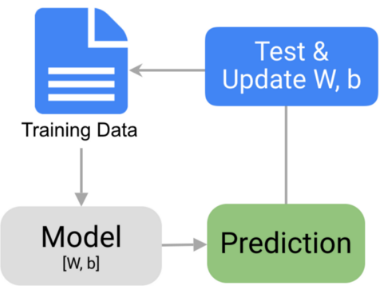
\includegraphics[width=\linewidth]{img/machine_learning_training.png}
\item Evaluation: Mit Evaluationsdaten testen ob Training gut genug.
\item Parameter Tuning: Experimentieren mit weitern Parameter um Training zu verbessern. «Hyperparameter»
\item Prediction: Model nutzen um nun mit anderen Daten eine Aussage machen zu können (Modell anwenden)
\end{enumerate}

\subsection{Bias and Variance}
\textcolor{myblue}{Bias}\\
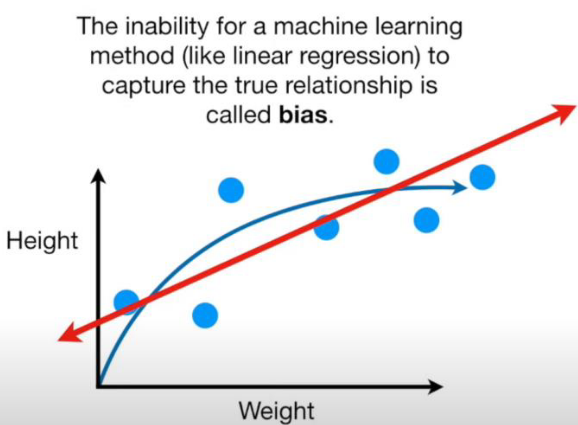
\includegraphics[width=\linewidth]{img/bias.png}
Da die gerade Linie nicht wie die \textit{wahre} Beziehung gekrümmt werden kann, weist sie einen relativ grossen Bias auf.
\textcolor{myblue}{Variance}
Differenz der Nähe der Daten (Sum of Squares) zwischen Test und Evaluationsdaten wird Varianz genannt.
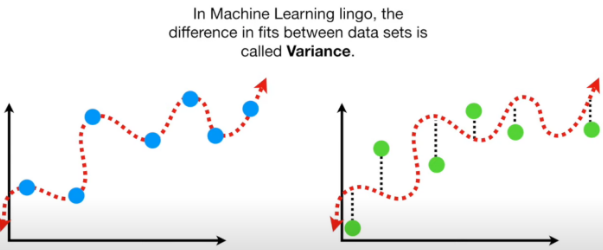
\includegraphics[width=\linewidth]{img/variance.png}